\begin{figure}
	\centering
	\begin{subfigure}{0.45\textwidth}
		\centering
		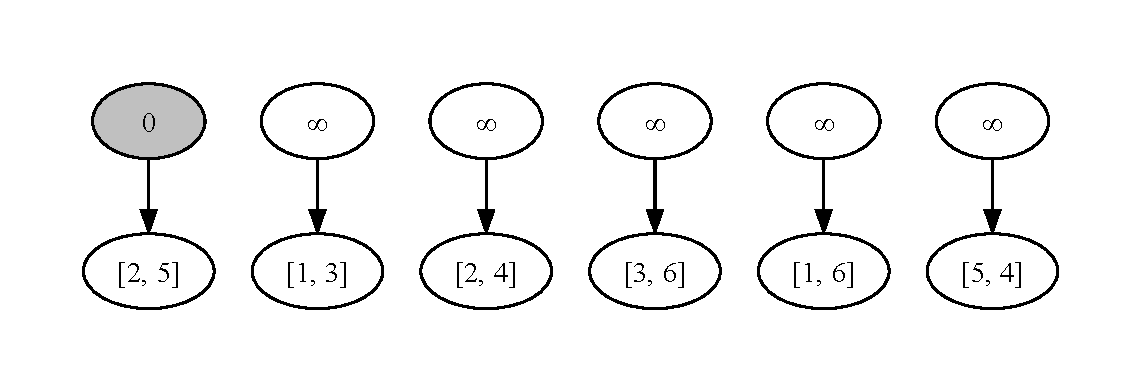
\includegraphics[width=\linewidth]{photos/diagrams/graphs/graph_state_1.pdf}
		\caption{State 1}
	\end{subfigure}
	\hfill
	\begin{subfigure}{0.45\textwidth}
		\centering
		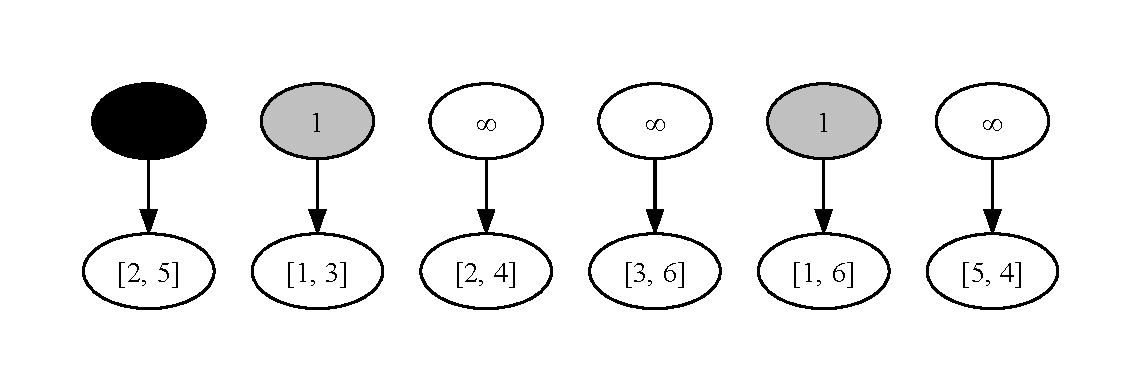
\includegraphics[width=\linewidth]{photos/diagrams/graphs/graph_state_2.pdf}
		\caption{State 2}
	\end{subfigure}
	\\
	\begin{subfigure}{0.45\textwidth}
		\centering
		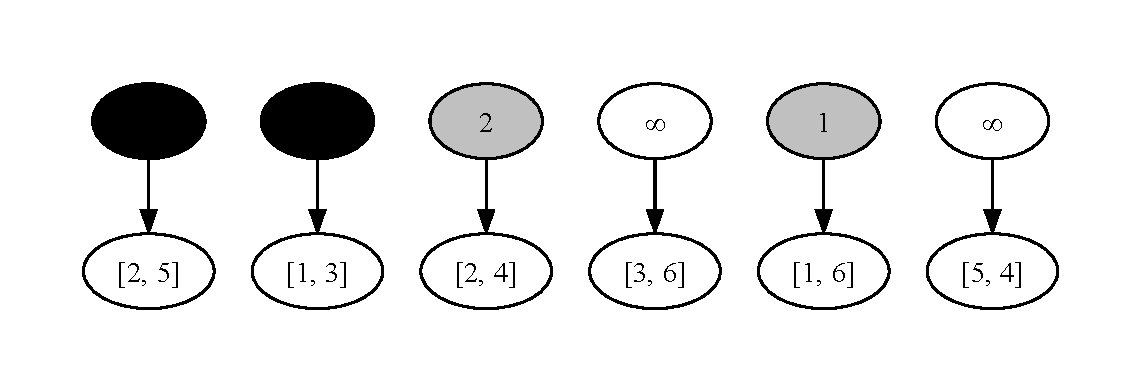
\includegraphics[width=\linewidth]{photos/diagrams/graphs/graph_state_3.pdf}
		\caption{State 3}
	\end{subfigure}
	\hfill
	\begin{subfigure}{0.45\textwidth}
		\centering
		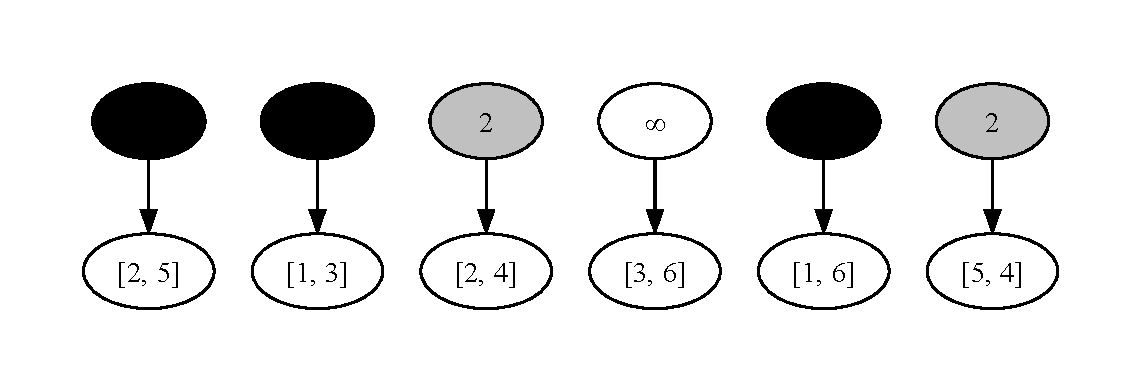
\includegraphics[width=\linewidth]{photos/diagrams/graphs/graph_state_4.pdf}
		\caption{State 4}
	\end{subfigure}
	% Repeat for all other graph states
	\caption{State of the graph after each dequeue.}
\end{figure}
